\begin{frame}
    \frametitle{Bag-of-Words}
    The early Bag-of-Words model is proposed by A.Zisserman and J. Sivic in 2003 \footcite{Sivic, J.; Zisserman, A., "Video Google: a text retrieval approach to object matching in videos," Computer Vision, 2003. Proceedings. Ninth IEEE International Conference on , vol., no., pp.1470,1477 vol.2, 13-16 Oct. 2003}. The main idea of their work is to represent an object as a set of invariant features, similar to words in a text document.

    The model was then improved by J. Philbin et al \footcite{Philbin, J.; Chum, O.; Isard, M.; Sivic, J.; Zisserman, A., "Object retrieval with large vocabularies and fast spatial matching," Computer Vision and Pattern Recognition, 2007. CVPR '07. IEEE Conference on , vol., no., pp.1,8, 17-22 June 2007} \footcite{Philbin, J.; Chum, O.; Isard, M.; Sivic, J.; Zisserman, A., "Lost in quantization: Improving particular object retrieval in large scale image databases," Computer Vision and Pattern Recognition, 2008. CVPR 2008. IEEE Conference on , vol., no., pp.1,8, 23-28 June 2008} with some advanced techniques such as \alert{soft assignments} and \alert{geometric verification} which was applied by the authors' work.
\end{frame}

\begin{frame}
    \frametitle{Bag-of-Words}
    \begin{figure}
    \begin{figure}{}
        \centering
        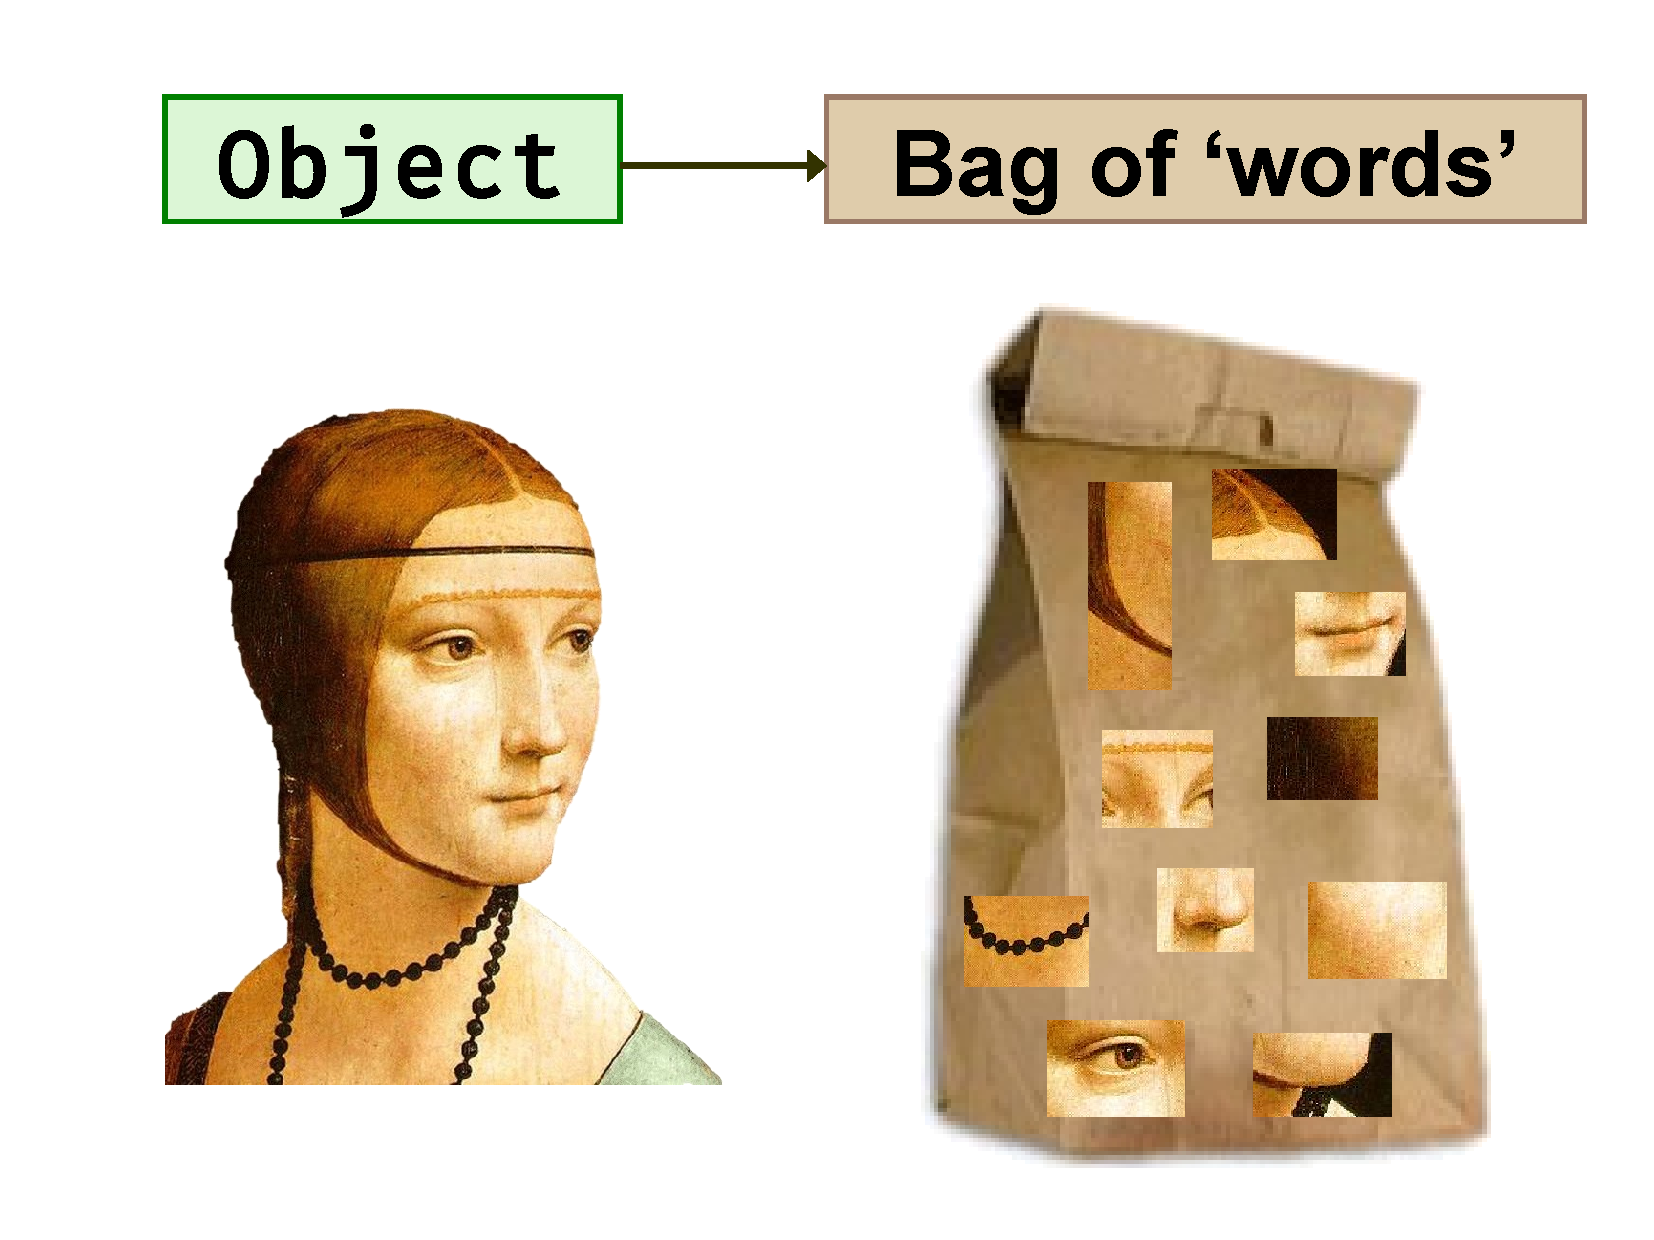
\includegraphics[width=3.5in]{images/bow.pdf}
        \caption{Bag-of-Words model\footcite{Slide credit: Rob Fergus, Classical Methods for Object Recognition}}
    \end{figure}
  \end{figure}
\end{frame}

\begin{frame}[fragile]
  \frametitle{Review of text retrieval}

  Common steps in text retrieval systems \footcite{R. Baeza-Yates and B. Ribeiro-Neto. Modern Information Retrieval. ACM Press, ISBN: 020139829, 1999}:

  \begin{itemize}
    \item Parse documents into words 
    \item Represent words by their sterms
    \item Reject common words by using stop list
    \item Represent each document by a vector of words' frequency (BoW)
    \item Retrieve a document by computing its BoW vector and returning documents with the closest vector
  \end{itemize}

\end{frame}

  
